%Input preamble
\input{preamble}
\let\counterwithout\relax
\let\counterwithin\relax
\definecolor{maroon}{HTML}{4B0082}
\usepackage{enumitem}


\begin{document}
\onehalfspacing

\noindent \textbf{Econ 900-03: Final Exam.}\\
\noindent Instructor: Jorge Luis García \\
\noindent e-mail: jlgarci@clemson.edu\\

\noindent \textbf{Read the Instructions.} 

\begin{enumerate}
	\item Starting time: 8:30 a.m.\ EST, 11/22/2021. Due date: 8:30 p.m.\ EST, 11/22/2021. This exam is comprised of three problems. The first problem is all theoretical and will require no code. Problems 2 and 3 contain both theoretical and empirical portions. Your submission will be comprised of three files. One file will contain answers to all of the theoretical parts in problems 1, 2, and 3. (Be sure to make it clear which part of each problem your are answering!) The other two files will be stata files. There will be one stata file containing all of the empirical work for problem 2 and one stata file containing all of the empirical work for problem 3. \textbf{E-mail Dr. Garcia} a scan with your theorical answers and name it ``yourlastname\_theory.'' \textbf{E-mail Dr. Garcia} a seperate code for the empirical portions of problem 2 and problem 3 with the names ``yourlastname\_empirical2'' and ``yourlastname\_empirical3''. \textbf{Include the three files in one e-mail titled ``your last name: final.''}
	\item You cannot talk to anyone about the exam during its duration. A qualified person with knowledge on the material of this class has taken this exam and has been able to answer it without clarification questions. If I detect that you  spoke to anyone during the exam, your grade for the class will be F.
\begin{enumerate}
	\item Theoretical Portions: Show your derivations as precisely as possible. Be concrete in your answers: For example, if I ask you for a statistic, you should indicate its degrees of freedom and these should be a number (not a function such as the ``the range of a matrix'').
	\item Empirical Portions: Be concise and clear when writing your code and comment in line when necessary. 
\end{enumerate}
	\item I am not able to answer emails during the week of the exam. I will send you the final grades prior to the last day of exam week. 
\end{enumerate}

\pagebreak
\noindent \textbf{Problem 1. Simple Instrumental Variables (10 points)} Consider a simple model to estimate the effect of personal computer (PC) ownership on college grade point average for graduating seniors at a large public university:
\begin{equation}
	GPA = \beta_0+\beta_1PC+u
\end{equation}
where PC is a binary varaible indication PC ownership.
\begin{enumerate}
	\item Why might PC ownership be correlated with u?
	\item Explain why PC is likely to be related to parents' annual income. Does this mean potential income is a good IV for PC? Why or why not?
	\item Suppose that, four years ago, the university gave grants to buy computers to roughly one-half of the incoming students, and the students who received grants were randomly chosen. Carefully explain how you would use this information to construct an instrumental variable for PC.
\end{enumerate}


\pagebreak
\setcounter{equation}{0}
\noindent \textbf{Problem 2. More Instrumental Variables (40 points)} For this exercise, use the data set -DahlLochner2012AER.dta- available on Canvas.Please be brief, but precise, in your answers. Note that you do not have to report more in the text than is asked for.\\

\noindent In a recent study published in the American Economic Review 2012, 102(5): 1927–1956, Dahl and Lochner (hereafter, DL) study how children’s school performance depends on family income. They posit the following model of the relationship:
\begin{equation}
	y_{ia}=x_i^{'}\alpha_a+w_{ia}^{'}\beta +\delta I_{ia}+u_{ia}
\end{equation}
where $y_{ia}$ and $I_{i,a}$ are the performance and family income, respectively, of child i at age a. $x_i$ and $w_{ia}$ are permanent and time-varying characteristics listed below, while $u_i$ reflects unobserved determinants of school performance.

\begin{enumerate}
	\item There are three performance measures in the data set -math-, -readingcomp- and -readingrecog-. Create a new variable -score- as the average of these variables, and standardize it to mean equal zero and standard deviation equal one.
	\item How much of the variation in -score- and -faminc- is coming from comparisons across individuals and how much is coming from comparisons within individuals over time?
	\item Graph the mean of -score- and -faminc- over time, and include a 95\% confidence interval. (Hint: You want to graph one observation per year( try -collapse- if you use Stata). Also, you need to generate new variables for the confidence interval using the standard error of the mean.)
	\item Estimate model (1) using OLS with -score- as the dependent variable, controlling for variables 9–26 (black hispanic male age agemom ed1age23 ed2age23 ed3age23 ed4age23 afqt afqt\_miss married spouseage spouseage\_miss famsize famsize\_miss sib1 sib3). Use robust standard errors. Interpret the coefficient on -faminc-.
	\item Do you think that the OLS-estimates may be biased? Explain your answer. In which direction do you think $\delta$ is biased?
\end{enumerate}

\noindent We have panel data with information on school performance of each child in several years. Assume that the error term above has an individual-specific component $\mu_i$ that is fixed over time, such that:
\begin{equation}
	u_{ia}=\mu_i+\epsilon_{ia}
\end{equation}
where $\epsilon_{ia}$ is random residual.


\begin{enumerate}[resume]
	\item Explain how you can use the panel structure of the data to get a more reliable estimate of $\delta$. Estimate this model using first differences for -score- and -faminc-. Include as control variables -black-, -hispanic-, -male-, -age-, -sib1-, and -sib3- (not differenced).
	\item Estimate the model with fixed effects (using -xtreg, fe- in case of Stata), including the same controls. (Why does Stata exclude the variables -black-, -hispanic-, and -male-?) How would you interpret the coefficient on these variables in the model in first differences?
	\item Why may we be worried about omitted variables bias also in the panel data models? (Hint: What is driving changes in family income?)
\end{enumerate}


\noindent While the EITC and other tax schedules do not generally vary with the child’s age in any given year, they do sometimes change over time (that is: with the age of the child, a). The following figure illustrates this for the 1986 and 1988 EITC in the US:

\begin{figure}[H]
		\centering
		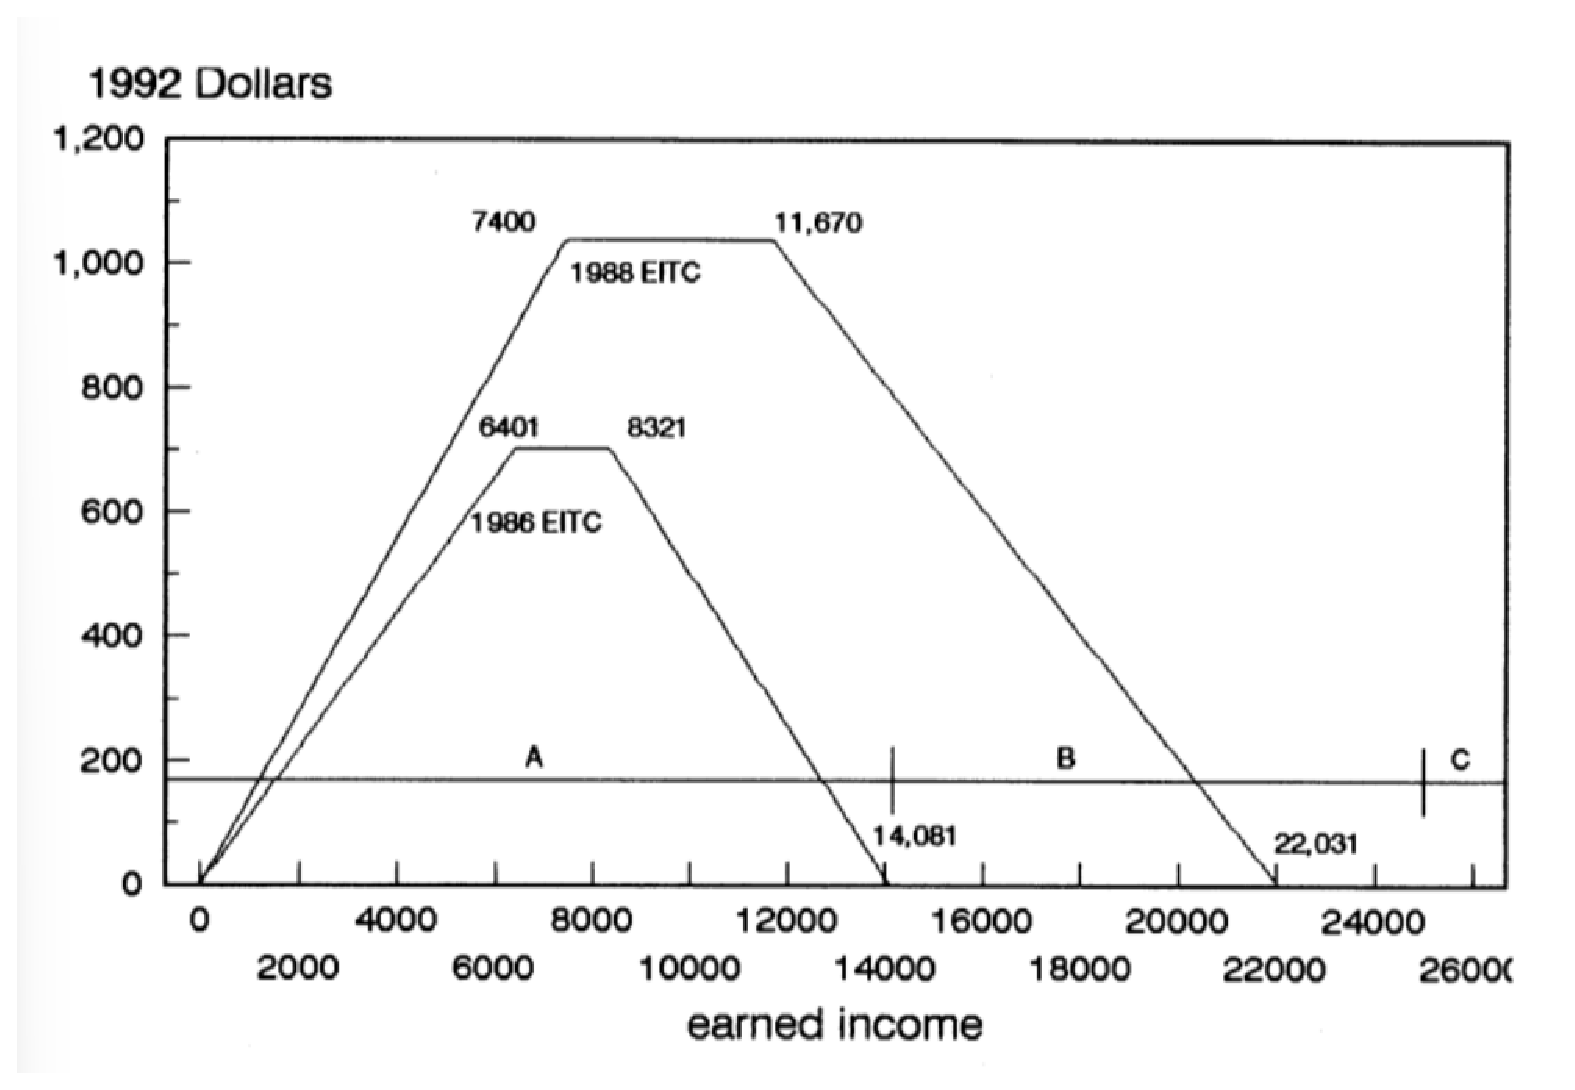
\includegraphics[width=.8\columnwidth]{graph1}
	\end{figure}

\noindent Total net family income is therefore given by:
\begin{equation}
	I_{ia}=P_{ia}+\chi_{ia}(P_{ia})-\tau_{ia}(P_{ia})
\end{equation}
where $P_{ia}$ is family income prior to taxes and transfers, and $\chi{ia}$ and $\tau_{ia}$ are the EITC and tax schedules, respectively.


\begin{enumerate}[resume]
	\item Explain why $\Delta\chi_{ia}(P_{i,a-1})=\chi_{ia}(P_{i,a-1}-\chi_{i,a-2}(P_{i,a-2})$ may be an instrument for $\DeltaI_{ia}$. Do you think $\Delta\chi_{ia}=\chi_{ia}(P_{i,a}-\chi_{i,a-2}(P_{i,a-2})$ would be a better or worse instrument for $\Delta I_{ia}$?
	\item In the data, $\chi_{ia}(P_{i,a})=eitc$ and $\chi_{ia}(P_{i,a-1}=eitcsim$. Estimate the model in first differences (as in 6 above) using $\Delta\chi_{ia}(P_{i,a-1})$ as an instrument.
	\item Should we be worried about $\Delta\chi_{ia}(P_{i,a-1})$ being a weak instrument?
\end{enumerate}


\noindent We may be worried that also $P_{i,a-1}$ is endogenous, since it may be associated with $P_{i,a}$ by e.g. serially correlated shocks. By including in our IV-model flexible controls for $P_{i,a-1}$, we may more plausibly incorporate in our instrument only the changes in $I_{ia}$ deriving from changes in EITC, and avoid incorporating general changes in family income.


\begin{enumerate}[resume]
	\item Reestimate the IV-model in 10 above, including as control variables the dummy -laborpart- and a fifth-order polynomial in -faminc\_L1-. Compare the estimates to those you got above.
	\item Using this final model, create a loop that estimates the model repeatedly, setting as the dependent variable one of the test score-variables: -score-, -math-, -readingcomp-, and -readingrecog-.
\end{enumerate}

\pagebreak


\setcounter{equation}{0}
\noindent \textbf{Problem 3. More Panel Methods (50 points)} The file -MATHPNL.dta- contains panel data on school districts in Michigan for the years 1992 through 1998. It is the district-level analogue of the school-level data used by Papke (2005). The response variable of interest in this question is $math4$, the percent age of fourth graders in a district receiving a passing score on a standardized math test. The key explanatory variable is $rexpp$, which is real expenditures per pupil in the district. The amounts are in 1997 dollars. The spending variable will appear in logarithmic form.

\begin{enumerate}
	\item Consider the static unobserved effects model:
	\begin{equation}
		math4_{it}=\delta_1 y93_t+...+\delta_6 y98_t+\beta_1log(rexpp_{it})+\beta_2log(enrol_{it})+\beta_3lunch_{it}+a_i+u_{it}
	\end{equation}
	where $enrol_{it}$ is total district enrollment and $lunch_{it}$ is the percentage of students in the district eligible for the school lunch program. (So $lunch_{it}$ is a pretty good measure of the district-wide poverty rate.) Argue that $\beta_1/10$ is the percentage point change in $math4_{it}$ when real per-student spending increases by roughly 10\%.
	\item Use first differencing to estimate the model in part (1). The simplest approach is to allow an intercept in the first-differenced equation and to include dummy variables for the years 1994 through 1998. Inter pret the coefficient on the spending variable.
	\item Now, add one lag of the spending variable to the model and reestimate using first differencing. Note that you lose another year of data, so you are only using changes starting in 1994. Discuss the coefficients and significance on the current and lagged spending variables.
	\item Obtain heteroskedasticity-robust standard errors for the first-differenced regression in part (3). How do these standard errors compare with those from part (3) for the spending variables? 
	\item Now, obtain standard errors robust to both heteroskedasticity and serial correlation. What does this do to the significance of the lagged spending variable?
	\item Verify that the differenced errors $r_{it}=\Delta u_{it}$, have negative serial corre lation by carrying out a test of AR(1) serial correlation.
	\item Based on a fully robust joint test, does it appear necessary to include the enrollment and lunch variables in the model?
\end{enumerate}

\noindent Consider the following specification:
\begin{equation}
	\begin{split}
		math4_{it}=\delta_1 y94_t+...+\delta_5 y98_t+\gamma_1log(rexpp_{it})+\gamma_2log(rexpp_{i,t-1}) \\ 
		+\phi_1log(enrol_{it})+\phi_2lunch_{it}+a_i+u_{it}
	\end{split}
\end{equation}
where the first available year (the base year) is 1993 because of the lagged spending variable.

\begin{enumerate}[resume]
	\item Estimate the model by pooled OLS and report the usual standard errors. You should include an intercept along with the year dummies to allow $a_i$ to have a nonzero expected value. What are the estimated effects of the spending variables? Obtain the OLS residuals $v\hat_{it}$. 
	\item Is the sign of the $lunch_{it}$, coefficient what you expected? Interpret the magnitude of the coefficient. Would you say that the district poverty rate has a big effect on test pass rates?
	\item Compute a test for AR(1) serial correlation using the regression $v\hat_{it}$ on $v\hat_{i,t-1}$. You should use the years 1994 through 1998 in the regression. Verify that there is strong positive serial correlation and discuss why.
	\item Now, estimate the equation by fixed effects. Is the lagged spending variable still significant? 
	\item Why do you think, in the fixed effects estimation, the enrollment and lunch program variables are jointly insignificant?
	\item Define the total, or long-run, effect of spending as $\theta_1=\gamma_1+\gamma_2$. Use the substitution $\gamma_1=\theta_1-\gamma_2$, to obtain a standard error for $\theta\hat_1$. [Hint: Standard fixed effects estimation using $log(rexpp_{it})$ and $z_{it}=log(rexpp_{i,t-1})-log(rexpp_{it})$ as explanatory variables should do it.]
\end{enumerate}

\pagebreak


\end{document}

